\clearpage
\section{Methodology}
\label{sec:Methodology}


%%%%%%%%%%%%%%%%%%%%%%%%%%%%%%%%%%%%%%%%%%%%%%%%%%%%%%%%%%%%%%%%%%%%%%%%%%%%%%%%%%%%%%%%%%%%%%%%%%%%%%%%%%%%%%%%%%%%%%%%%%%%%%%%%%%%%%%%%%%%%%%%%%%%%%%%%%%%%%%%%%%%%%%%%%%%%%%%%%%%%%%%%%%%%%%%%%%%%%%%%%%%%%%%%%%%%%%%%%%%%%%%%%%%%%%%%%%%%%%%%%%%%%%%%%%%%%%%%%%%%%%%%%%%%%%%%%%%%%%%%%%%%%%%%%%%%%%%%%%%%%%%%%%%%%%%%%%%%%%%%%%%%%%%%%%%%%%%%%%%%%%%%%%%%%%%%%%%%%%%

\subsection{Flow Problem of Interest}
\label{sec:Flow problem of interest}
To understand the effect of oscillating wall flow control to the effect of the flow, a case must be formulated as an example case. Generally, the case used is a canonical flow problem, which the information and data are abundantly accessible and can easily compared to one and another. Therefore, the turbulence phenomena can be throughly examined. In this study, a simple double periodic channel flow problem is used to be analysed for the oscillating wall flow control problem. Double periodic channel flow cases utilises periodic boundary conditions on two sets of planes: spanwise and streamwise planes. 

The first thing to do when simulating a double periodic channel flow problem is to determine the requirement of the channel flow domain size. The size of the domain must be meticulously determined to minimise the computational expenses but ensuring all of the necessary turbulence structures are captured appropriately. The minimum size of the double periodic channel flows are commonly referred as the minimal flow unit \cite{Jimenez1991}, shown in Figure \ref{fig:jimenezmfu}.

\begin{figure}[ht]
	\centering
	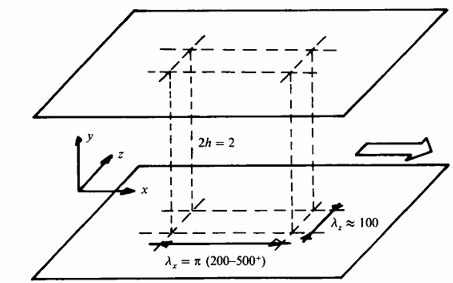
\includegraphics[width=0.6\linewidth]{Figures/JimenezMFU}
	\caption{Minimal Flow Unit of a Double Periodic Channel Flow~\cite{Jimenez1991}}
	\label{fig:jimenezmfu}
\end{figure}

The length of the minimal flow unit is defined in a wall flow unit, denoted by the (+) sign. The (+) sign is a normalisation of the quantity using the turbulent boundary layers, formulated as:

\begin{equation}
	+ = \frac{\nu}{u_\tau}
\end{equation}

Where $u_\tau$ is a function of wall friction, defined as \cite{Pope2000}:

\begin{equation}
	u_\tau = \sqrt{\frac{\tau_w}{\rho}}
\end{equation}

$\tau_w$ is related to the Reynolds numbers and the velocity gradient to the normal direction, stated as \cite{Daniel2017}:
\begin{equation}
	\tau_{w} = \frac{\partial u}{\partial y} Re
\end{equation}

$Re$ is the dimensionless number which displays the ratio between the inertial and viscous forces, expressed as \cite{NASA_Re}:
\begin{equation}
	Re = \frac{v \delta}{\nu}
\end{equation}

For study in turbulence, friction Reynolds numbers are more commonly used due to its relevance to the near wall turbulence. The equation of the friction Reynolds number is displayed below \cite{Pope2000}.
\begin{equation}
	Re_\tau = \frac{u_\tau \delta}{\nu} \approx 0.09 (2Re)^{0.88} 
\end{equation}

For the base case, the Reynolds number are defined as $Re_\tau = 180$. The quantity is chosen due to the availability of DNS channel flow data \cite{Lee2015} and the data from Xcompact3D \cite{Bartholomew2020}. The fluid properties data is shown in the Table \ref{tab:fluprop} below.

\begin{table}[ht]
	\caption{Fluid Properties}
	\label{tab:fluprop}
	\centering
	\begin{tabular}{ccccc}
		\hline
		{$\boldsymbol{Re_\tau}$} & \textbf{Re} & \textbf{u} & {$\boldsymbol{\rho}$} & {$\boldsymbol{\nu}$} \\ \hline
		180               & 2819.294    & 1          & 1               & 0.00035        \\ \hline
	\end{tabular}
\end{table}
 



\subsection{Theoretical Background}
\label{sec:Governing equations SECTION}




\subsubsection{Governing Equations of Incompressible Fluid Flow}
\label{sec:Governing equations comp}

In a general fluid flow, there are two equations that are used for the equation\cite{Konoszy2023}. The first, continuity equation is expressed as:
\begin{equation}
	\frac{\partial P}{\partial t} + \nabla(\rho \mathbf{u}) = 0
\end{equation}

The second, is the momentum equation, which are commonly mentioned as the Navier-Stokes equation, is expressed as:

\begin{equation}
	\underbrace{\rho\frac{\partial \mathbf{u}}{\partial t}}_{\rm I.} + \underbrace{\rho(\mathbf{u}\cdot \nabla)\mathbf{u}}_{\rm II.} = \underbrace{\rho\mathbf{g}}_{\rm III.} - \underbrace{\nabla P}_{\rm IV.} + \underbrace{\mu \nabla^2 \mathbf{u}}_{\rm V.} + \underbrace{\frac{\mu}{3}\nabla(\nabla \mathbf{u})}_{\rm VI.}
\end{equation}

Where
\begin{equation}
	\mathbf{u} = u \mathbf{e_x} + v \mathbf{e_y} + w \mathbf{e_z}
\end{equation}

There are six members in a full on Navier-Stokes Equation. The first member is the unsteady term, showing the change of the fluid velocity over time. The second member is the convective-advective term, showing the transport of properties in the flow. The third term, gravity force field, displays the effect of gravity in the flow, The fourth term is the pressure gradient, showing the change of pressure in the fluid. The fifth term, the diffusion term, determines how the viscous diffusion and dissipation affecting the flow. Lastly, the sixth term, shows the compressibility effect due to the viscous terms. 

In a low Reynolds number case such as defined in Section \ref{sec:Flow_prob_interest}, the fluid becomes incompressible, which transforms both governing equations\cite{Konoszy2024}. For the continuity equation, the expression simplifies into:

\begin{equation}
	\nabla \mathbf{u} = 0
\end{equation}

On the other hand, the momentum equation changes by dropping the compressibility term. Additionally, the momentum equation can be modified by normalising every term to density, as density remains constant in incompressible flow.

\begin{equation}
	\frac{\partial\mathbf{u}}{\partial t}+(\mathbf{u}\cdot\nabla)\mathbf{u} = \mathbf{g} - \frac1\rho \nabla P + \nu \nabla^2 \mathbf{u}
\end{equation}



\subsubsection{Fractional Step Method}
\label{sec:Frac_step}
In incompressible flow, the density remains constant while the pressure changes. Therefore, the equation of state is not applicable \cite{Konoszy2024}, hence pressure and velocity equation must be calculated together in a coupled equation. In Xcompact3D, Chorin's Fractional Step Method is used \cite{Laizet2024}. In Fractional Step method, there are three steps that is conducted to couple the pressure and velocity variables \cite{Westra2002}. The first step utilises intermediate velocity field, which is expressed as:
\begin{equation}
	\mathbf{u}^* = \mathbf{u}^{n} + \Delta t \left[\mathbf{g}+\nu\nabla^2\mathbf{u}-(\mathbf{u}\nabla)\mathbf{u}\right]^{(n)}
\end{equation}
Then, the second step is conducted to solve the pressure equation as follows:
\begin{equation}
	\nabla^2 P^{n+1} = \frac{\rho}{\Delta t}\left[\nabla\mathbf{u^*}\right]
\end{equation}
Finally, the third step is to update the velocity.
\begin{equation}
	\mathbf{u}^{n+1}=u^*-\frac{\Delta t}{\rho}\nabla P^{n+1}
\end{equation}


\subsubsection{Spatial Discretisation}



\subsubsection{Temporal Discretisation}
\label{sec:temp_disc}
Other than the spatial discretisation, temporal discretisation must also be applied to calculation so the numerical simulation can be progressed to the next time step. For nearly all of the time discretisation, the third-order Adam-Bashforth equation is used. The third order Adam-Bashforth scheme is an explicit scheme that uses one equation to progress the time step of the calculation \cite{Durran1991}, displayed as:
\begin{equation}
	\phi^{n+1} - \phi^{n} = \frac{\Delta t}{12} [23F^{n} - 16F^{n+1}+5F^{n-2}]
\end{equation}

Where
\begin{equation*}
	\begin{gathered}
		F^n = \mathbf{u}^n \phi^n\\
		F^{n-1} = \mathbf{u}^{n-1} \phi^{n-1}\\
		F^{n-2} = \mathbf{u}^{n-2} \phi^{n-2}\\
		\label{eq:Fhalf}
	\end{gathered}
\end{equation*}

For the diffusion term in the wall-normal direction, the implicit Crank-Nicolson equation is also used for the time discretisation. The temporal discretisation for the y-diffusion term can be expressed as:

\begin{equation}
	\left( \nu \frac{\partial^2 v}{\partial y^2} \right)^{n+\frac{1}{2}} = \frac{1}{2} \left( \nu \frac{\partial^2 v^{n+1}}{\partial y^2} + \nu \frac{\partial^2 v^n}{\partial y^2} \right)
\end{equation}



\subsection{Computational Procedures}
\label{sec:Computational procedures}
 

\subsubsection{Grid Generation}
\label{sec:Gridgen}
For the entirety of the study, the cartesian structured grid is used. The entire model is discretised into a system of hexahedral-shaped elements with eight nodes connecting to each other \cite{Yeoh2010}. In a simple canonical flow as this study, the structured hexahedral grid is favoured due to the the efficiency of the shape in terms of filling the spaces, as well as the ability of minimising diffusion when transfering the properties from an element to another \cite{ANSYS2020}. Additionally, the simple connectivity of the elements makes the grid model simple to program \cite{TU2018125}.

To capture the near-wall turbulence, the size of the grid near the wall must be decreased. However, just uniformly decrease the size of the grid may cause an unnecessary computational expense as the flow on the centre of the channel flow do not have substantial gradient or turbulence structures. To compensate the problem, a stretching algorithm is introduced in the Xcompact3d program \cite{Laizet2009}, developed from \cite{Cain1984} and \cite{Avital2000}. First, the domain must be expressed in physical coordinate y and computational coordinate s.

\begin{equation}
	y = h(s), 0\le s \le 1, 0 \le y \le L_y
\end{equation}

The y-height of each members can be defined as
\begin{equation}
	h = \frac{L_y \sqrt{\beta}}{\gamma \sqrt{\alpha} \sqrt{\alpha \beta} + 1} \left\{ \tan^{-1} \left( \frac{\sqrt{\alpha \beta} + 1 \tan (\pi (\gamma s + \delta))}{\sqrt{\alpha}\sqrt{\beta}} \right) + \pi \left[ H \left( s - \frac{1 - 2\delta}{2\gamma} \right) + H \left( s - \frac{3 - 2\delta}{2\gamma} \right) \right] - \tan^{-1} \left( \frac{\sqrt{\alpha \beta} + 1 \tan (\pi \delta)}{\sqrt{\alpha} \sqrt{\beta}} \right) \right\}
	\label{eq:stretchingeq}
\end{equation}

On a default channel case in Xcompact3d, the refinement are conducted solely for the wall. Therefore, $\gamma = 1$ and $\delta = \frac12$. For all the case, $\beta$ is set to 0.259065151.





\subsubsection{Numerical Simulations: Settings}
\label{sec:Numerical simulations.Settings}


\subsubsection{Numerical Simulations: Simulations Campaign}
\label{sec:Numerical simulations.Simulations campaign}








